


\begin{document}

This section details the experimental implementation of the two differential amplifiers, the resistively loaded and active loaded. The power supplies and analysis were implemented using the Digilent Analog Discovery kit.

\subsection{Resistively loaded differential amplifier}
The resistively loaded amplifier was constructed in two different ways. The first was constructed using a cascode current mirror and the other was constructed using a simple current mirror.

\subsubsection{Cascode current mirror}

The experimental circuit for the resistively loaded differential amplifier is shown in Figure \ref{fig:ResLoadExp} below.



\begin{figure}[H]
    \begin{center}
    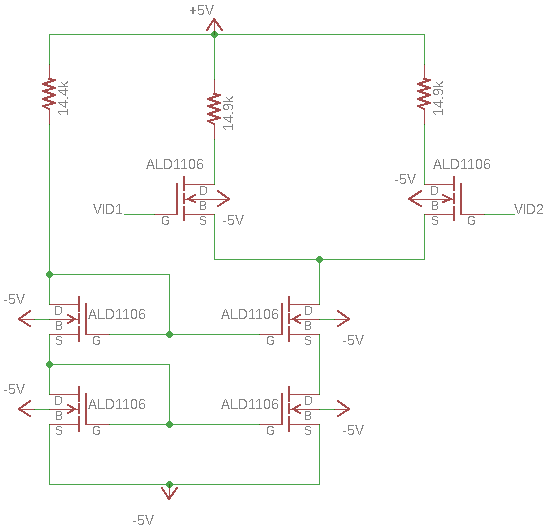
\includegraphics[scale=.75]{ExperimentalImplementation/ResLoadedExp.png}
    \caption{Experimental active load differential amplifier}
    \label{fig:ResLoadExp}
    \end{center}
\end{figure}

The drain resistances were measured to be 14.9kHz for each branch

Compared to the simulated circuit for the resistively loaded differential amplifier, that values needed to be changed in order to meet specifications. The values of the node voltages and altered component values are seen in Table \ref{tab:ExpResLoadValues} below. 

\begin{table}[H]
\centering
\caption{Experimental resistively loaded differential amplifier values}
\label{tab:ExpResLoadValues}
\begin{tabular}{|c|c|}
\hline
\multicolumn{2}{|c|}{\begin{tabular}[c]{@{}c@{}}Simulated resistively loaded \\ differential amplifer\end{tabular}} \\ \hline
Components/Nodes                                              & Values                                              \\ \hline
$V_{ref_1}$                                                   & -3.13V                                               \\ \hline
$V_{ref_2}$                                                   &  -0.62V                                                   \\ \hline
$I_{bias}$                                                    &   397$\mu$A                                                  \\ \hline
$I_{ref_1}$                                                   &   197$\mu$A                                                  \\ \hline
$I_{ref_2}$                                                   &   196$\mu$A                                                  \\ \hline
\end{tabular}
\end{table}




The VTC for this topology can be seen in Figure \ref{fig:resloVTC}.
\begin{figure}[H]
    \begin{center}
    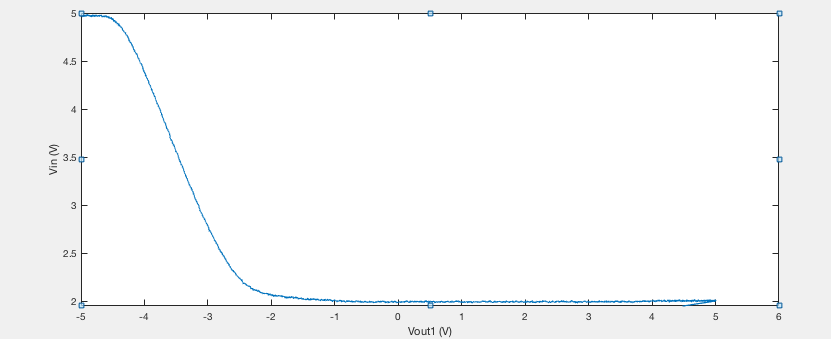
\includegraphics[scale=.45]{ExperimentalImplementation/VTC_res_cascode.png}
    \caption{Experimental VTC of cascode resistive load amplifier}
    \label{fig:resloVTC}
    \end{center}
\end{figure}
The range of operation can be seen by the central linear region, this region is the region of saturation for this set up. The differential gain for both the single ended and double ended outputs can be seen in in Figure \ref{fig:resloadAd}.


\begin{figure}[H]
    \centering
    \begin{subfigure}[b]{0.45\textwidth}
        \centering
        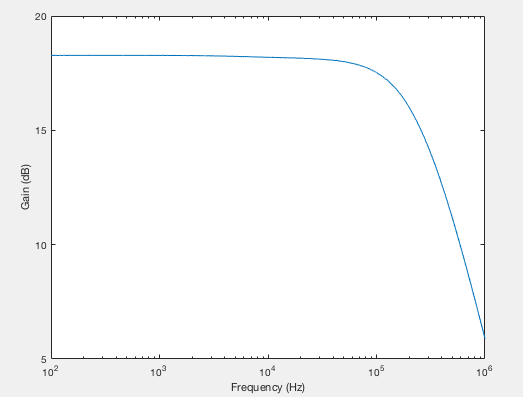
\includegraphics[width=\textwidth]{ExperimentalImplementation/Ad_cascode_res_double.png}
        \caption{Ad, double ended}
        \label{fig:blue_led}
    \end{subfigure}
    \hfill
    \begin{subfigure}[b]{0.45\textwidth}
        \centering
        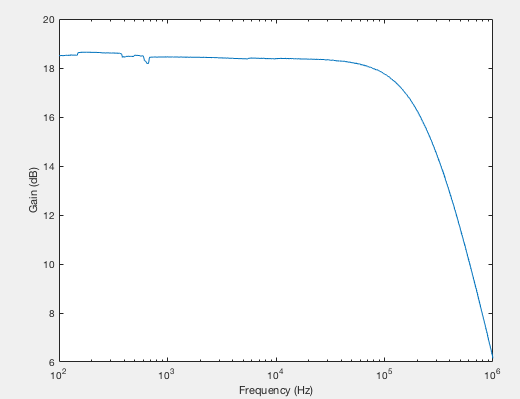
\includegraphics[width=\textwidth]{ExperimentalImplementation/Ad_cascode_res_single.png}
        \caption{Ad, single ended}
        \label{fig:blue_led}
    \end{subfigure}
    \caption{Differential gain, Ad, Cascode resistive load}
    \label{fig:resloadAd}
\end{figure} 

It can be seen that the single ended operated slightly better than the double ended. The common mode gain measured at 100mV can be seen in Figure \ref{fig:Acmreslo}.

\begin{figure}[H]
    \centering
    \begin{subfigure}[b]{0.45\textwidth}
        \centering
        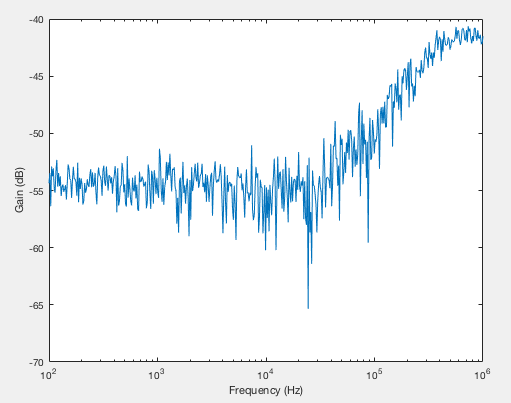
\includegraphics[width=\textwidth]{ExperimentalImplementation/Acm_100m_double.png}
        \caption{Acm, double ended}
        \label{fig:blue_led}
    \end{subfigure}
    \hfill
    \begin{subfigure}[b]{0.45\textwidth}
        \centering
        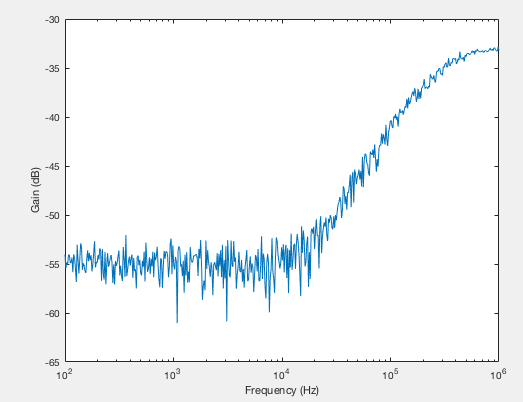
\includegraphics[width=\textwidth]{ExperimentalImplementation/Acm_100msingle.png}
        \caption{Acm, single ended}
        \label{fig:blue_led}
    \end{subfigure}
    \caption{Common mode gain, Acm, cascode resistive load}
    \label{fig:Acmreslo}
\end{figure} 

The measurement was repeated for 1V as well, which can be seen in Figure \ref{fig:resloadAcm1V} 

\begin{figure}[H]
    \centering
    \begin{subfigure}[b]{0.45\textwidth}
        \centering
        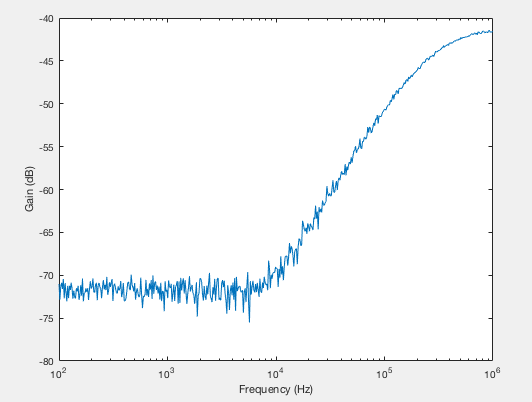
\includegraphics[width=\textwidth]{ExperimentalImplementation/Acm_1_double.png}
        \caption{Acm, double ended}
        \label{fig:blue_led}
    \end{subfigure}
    \hfill
    \begin{subfigure}[b]{0.45\textwidth}
        \centering
        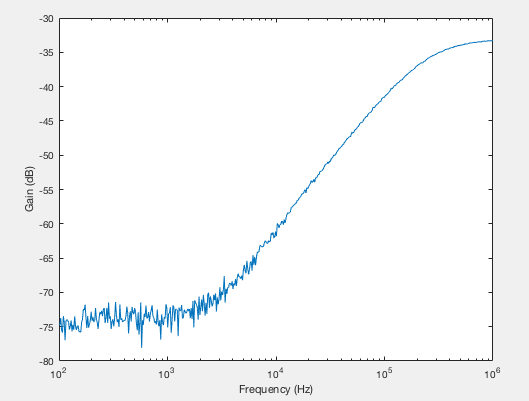
\includegraphics[width=\textwidth]{ExperimentalImplementation/Acm_1_single.png}
        \caption{Acm, single ended}
        \label{fig:blue_led}
    \end{subfigure}
    \caption{Common mode gain, Acm, cascode resistive load}
    \label{fig:resloadAcm1V}
\end{figure} 

The 1V clearly had less noise, which is ideal. The trade off, however, is this can saturate the differential gain. From these measurements the CMRR was found by combining the datasets for Ad and Acm in Matlab and can be seen in Figure \ref{fig:CMRR_cascode}.


\begin{figure}[H]
    \centering
    \begin{subfigure}[b]{0.45\textwidth}
        \centering
        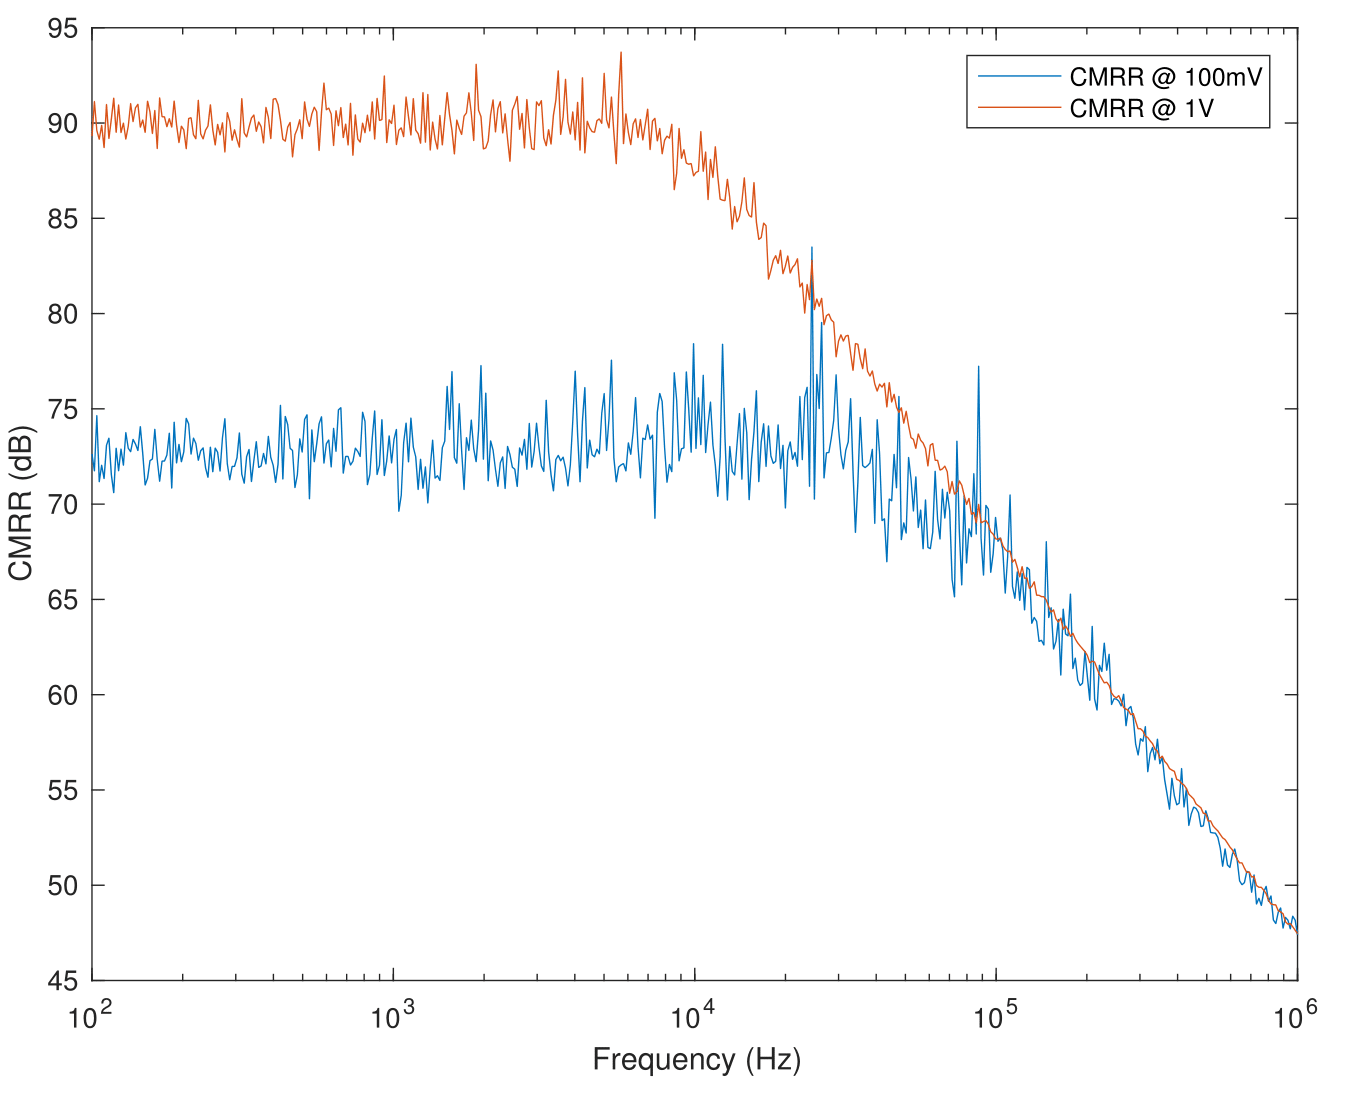
\includegraphics[width=\textwidth]{ExperimentalImplementation/CMRR_cascode_resist_double.png}
        \caption{CMRR double ended}
        \label{fig:blue_led}
    \end{subfigure}
    \hfill
    \begin{subfigure}[b]{0.45\textwidth}
        \centering
        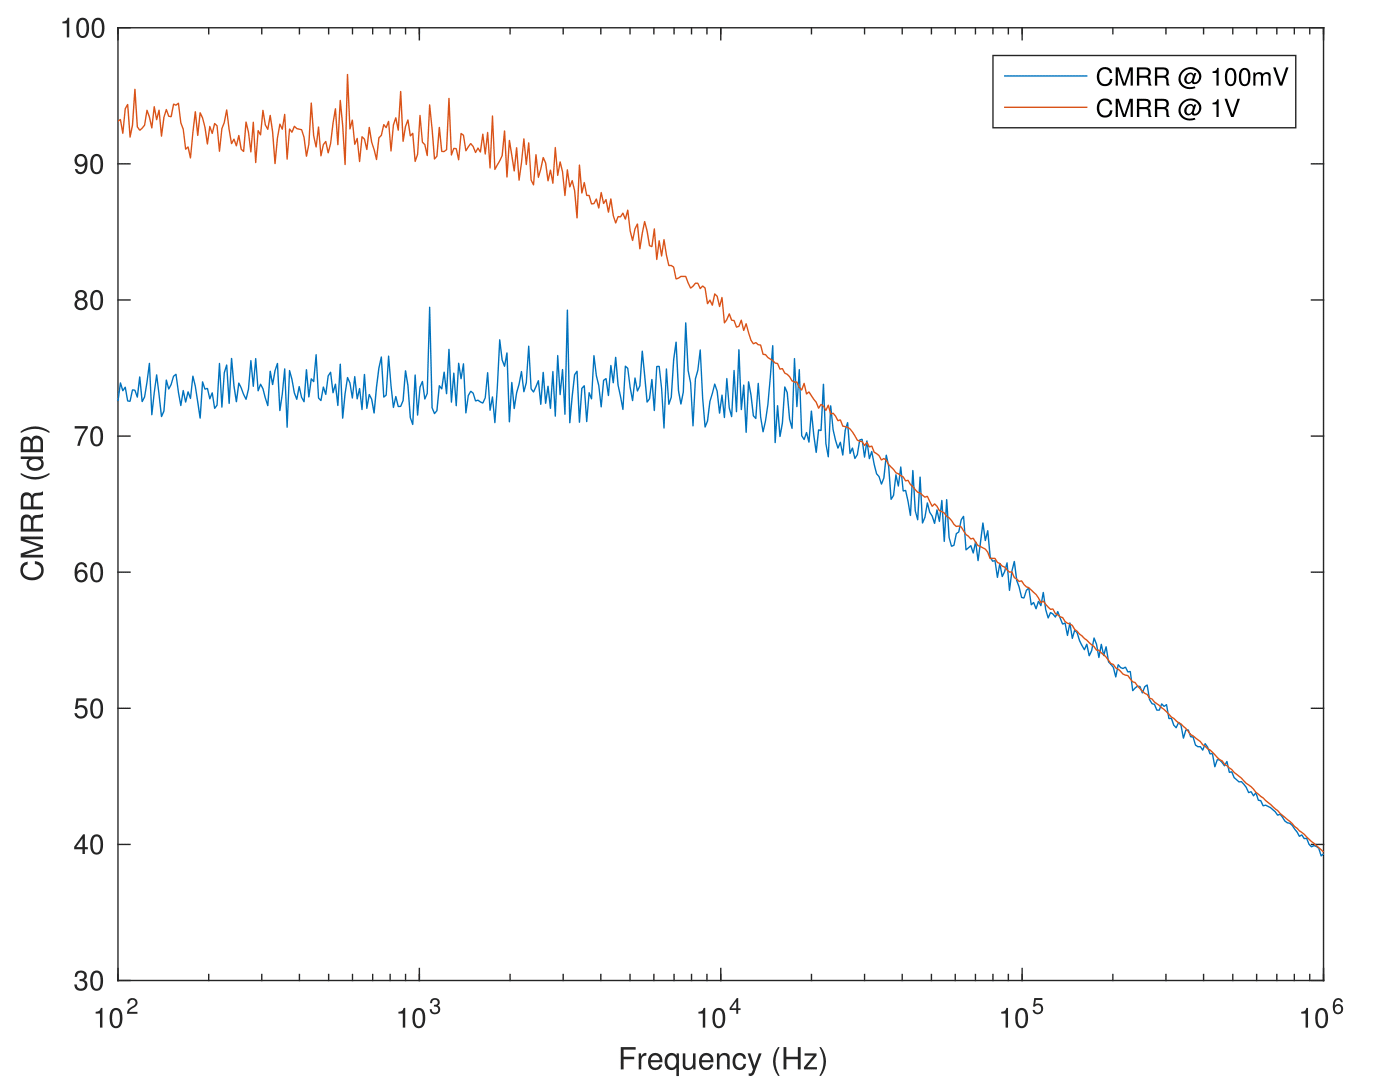
\includegraphics[width=\textwidth]{ExperimentalImplementation/CMRR_cascode_single_resist.png}
        \caption{CMRR single ended}
        \label{fig:blue_led}
    \end{subfigure}
    \caption{CMRR cascode resistive load}
    \label{fig:CMRR_cascode}
\end{figure} 

The amplifier produced a much higher CMRR, approximately 15dB, for the 1V input.









%%%%%SIMPLE
\subsubsection{Simple current mirror}

The simple current mirror was created by simply removing the conducting transistor N3 from the cascode. The DC bias conditions can be seen in Table \ref{tab:ExpResLoadValuesSimple}





\begin{table}[H]
\centering
\caption{Experimental resistively loaded differential amplifier, simple current mirror}
\label{tab:ExpResLoadValuesSimple}
\begin{tabular}{|c|c|}
\hline
\multicolumn{2}{|c|}{\begin{tabular}[c]{@{}c@{}}Simulated resistively loaded \\ differential amplifer\end{tabular}} \\ \hline
Components/Nodes                                              & Values                                              \\ \hline
$V_{ref_1}$                                                   & -3.09V                                               \\ \hline
$I_{bias}$                                                    &   398$\mu$A                                                  \\ \hline
$I_{ref_1}$                                                   &   202$\mu$A                                                  \\ \hline
$I_{ref_2}$                                                   &   203$\mu$A                                                  \\ \hline
\end{tabular}
\end{table}

The change to simple did little to impact the DC bias conditions of the circuit. The VTC of the simple current mirror mode can be seen in Figure \ref{fig:VTCsimple}.
\begin{figure}[H]
    \begin{center}
    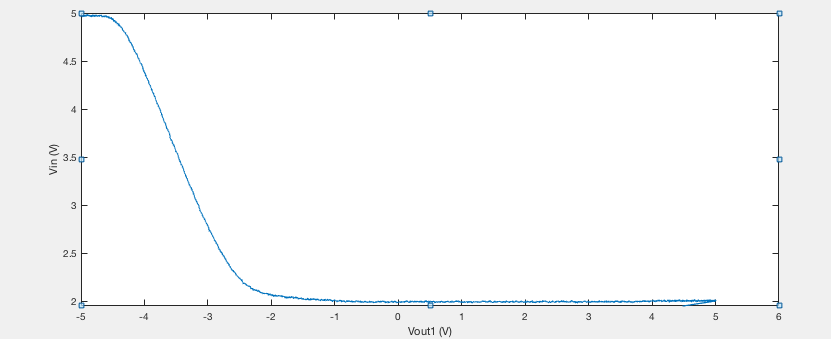
\includegraphics[scale=.45]{ExperimentalImplementation/VTC_res_cascode.png}
    \caption{Experimental VTC of simple current mirror resistive load amplifier}
    \label{fig:VTCsimple}
    \end{center}
\end{figure}
The compliance range is wider than that of the cascode, discussion of this can be found in the Discussion section. The differential gain for the simple current mirror case can be seen in Figure \ref{fig:resloadAdsimple}.

\begin{figure}[H]
    \centering
    \begin{subfigure}[b]{0.45\textwidth}
        \centering
        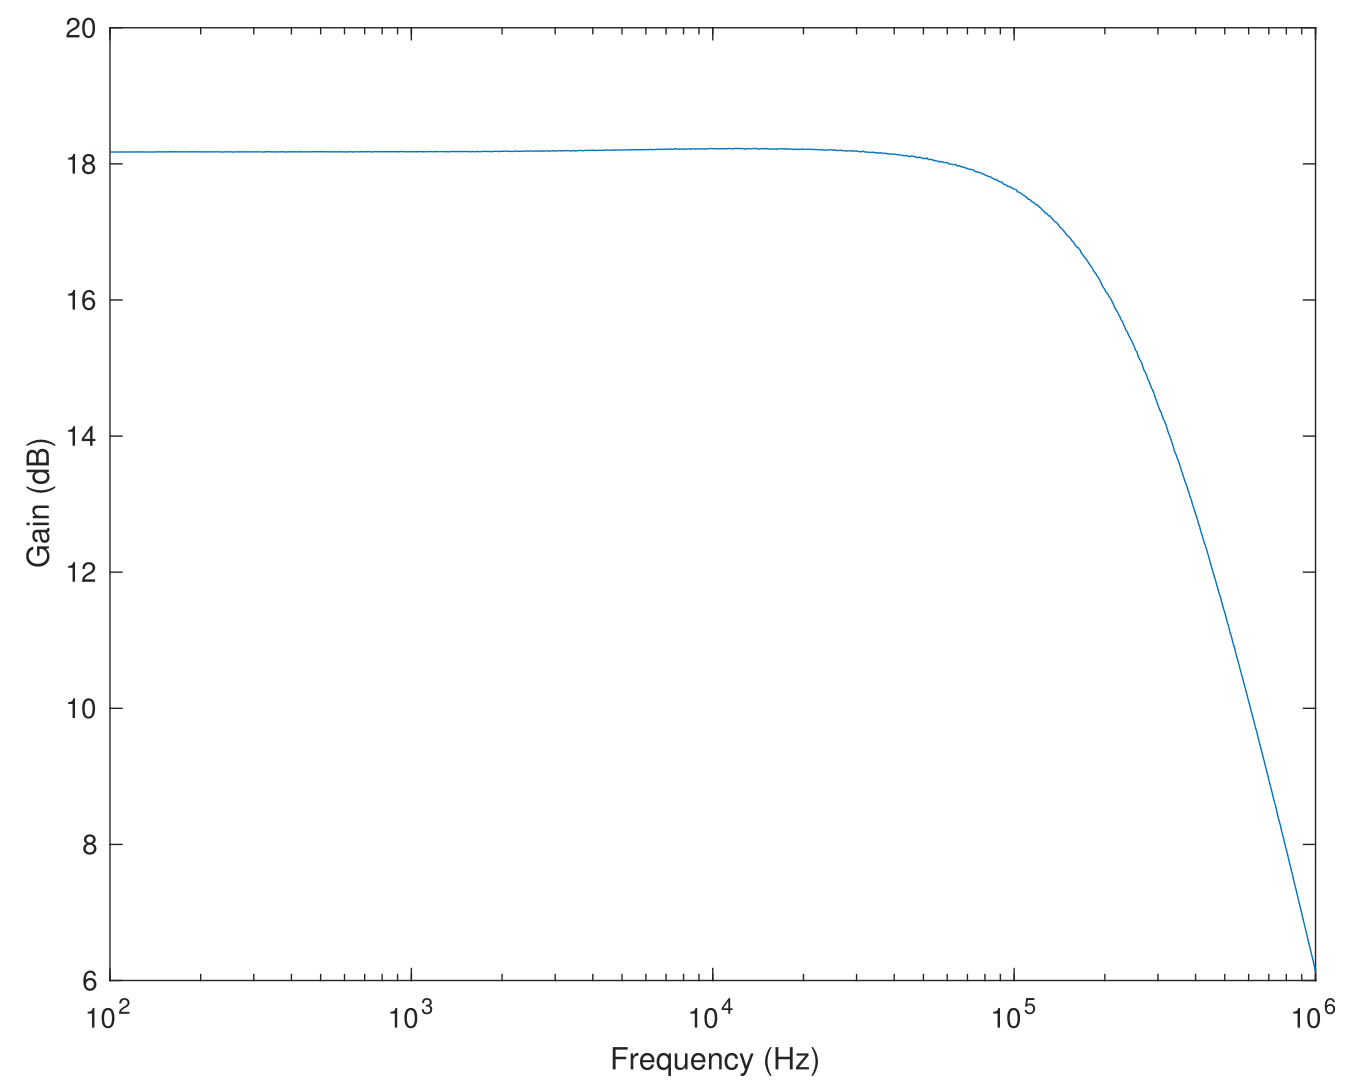
\includegraphics[width=\textwidth]{ExperimentalImplementation/Resist_Ad_simple_doubleended.png}
        \caption{Ad, double ended}
        \label{fig:blue_led}
    \end{subfigure}
    \hfill
    \begin{subfigure}[b]{0.45\textwidth}
        \centering
        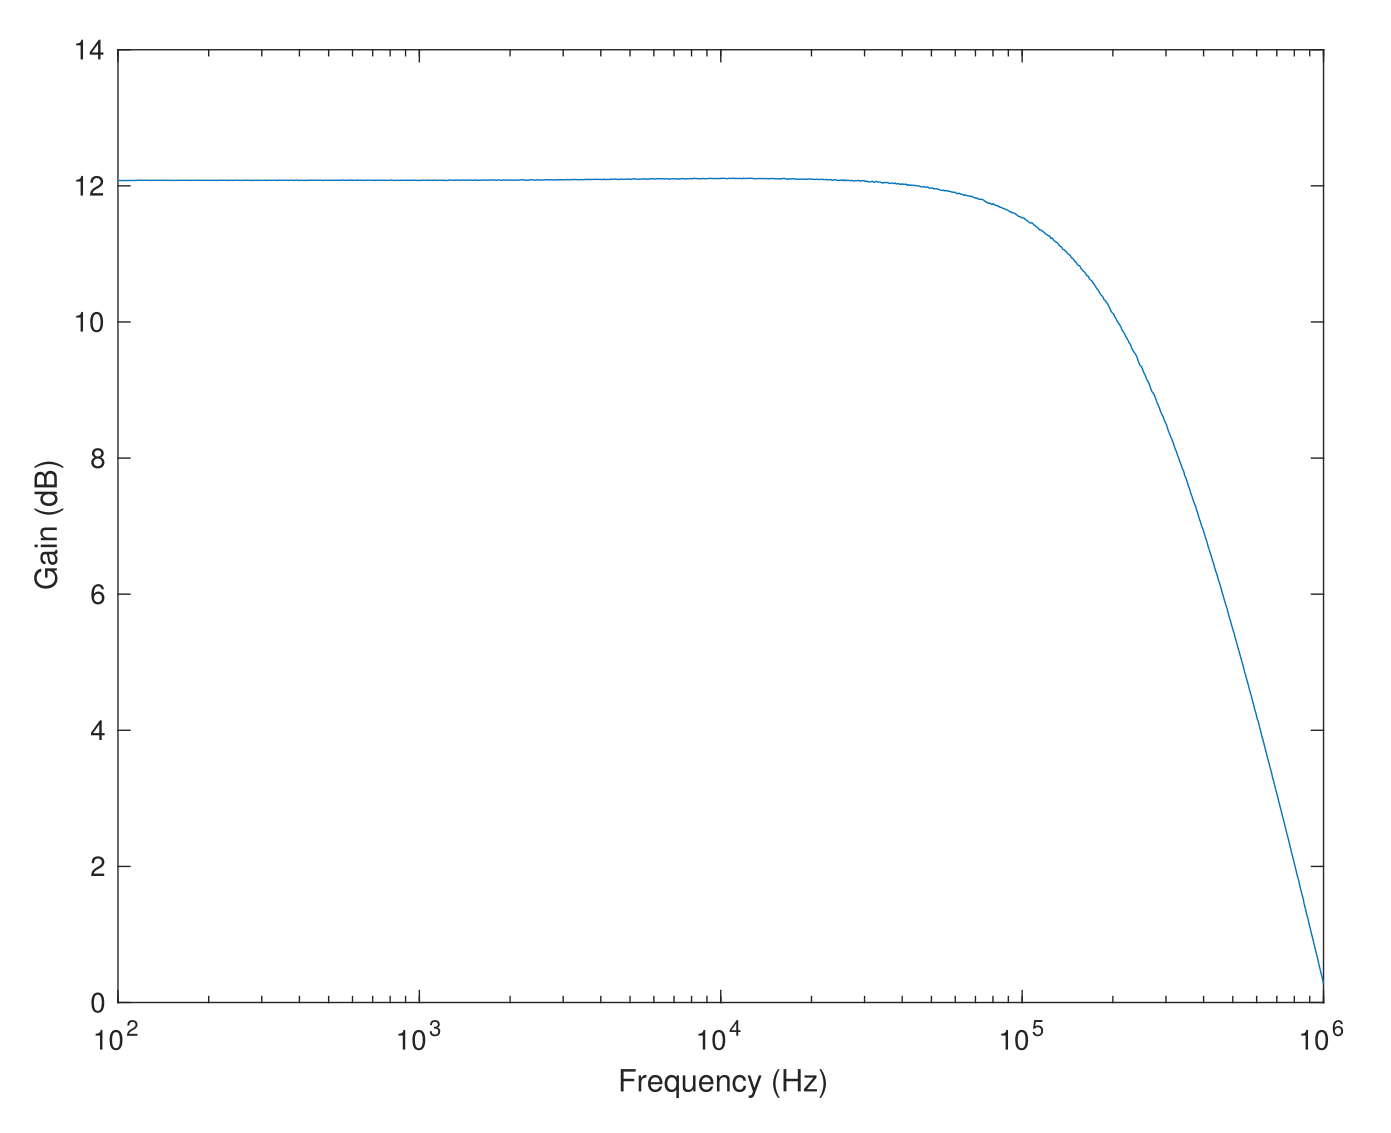
\includegraphics[width=\textwidth]{ExperimentalImplementation/Ad_resist_simple_singleended.png}
        \caption{Ad, single ended}
        \label{fig:blue_led}
    \end{subfigure}
    \caption{Differential gain, Ad, simple resistive load}
    \label{fig:resloadAdsimple}
\end{figure} 

It can be seen that the single ended operated slightly better than the double ended. The common mode gain measured at 100mV can be seen in Figure \ref{fig:Acmressimple}.

\begin{figure}[H]
    \centering
    \begin{subfigure}[b]{0.45\textwidth}
        \centering
        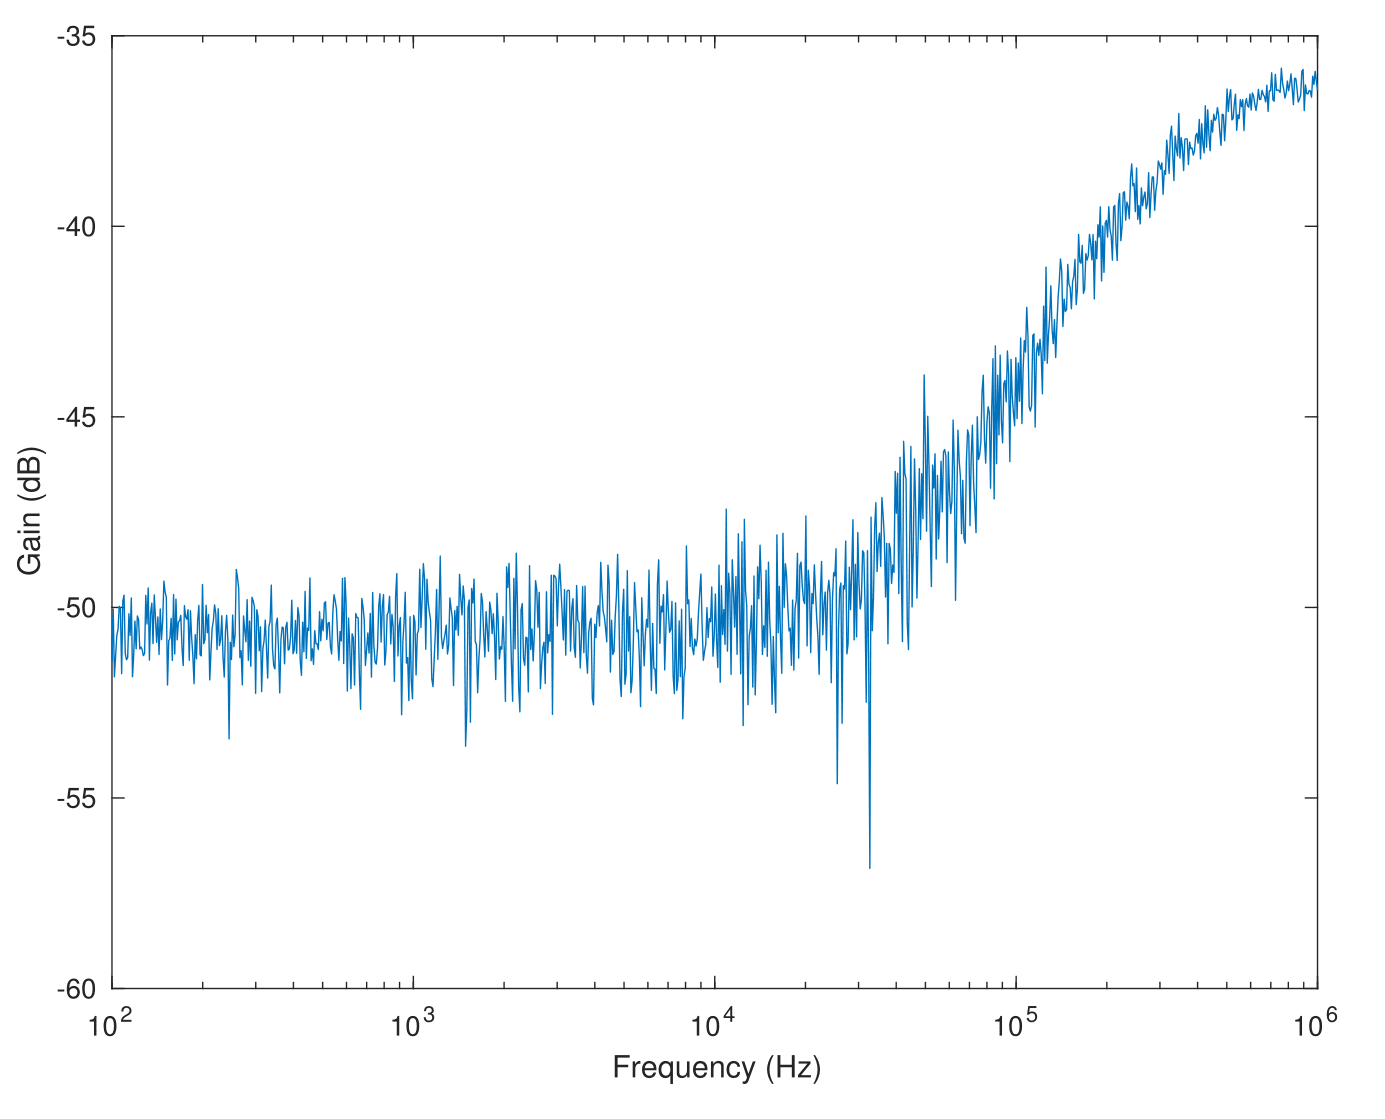
\includegraphics[width=\textwidth]{ExperimentalImplementation/Acm_resistive_double_ended_100m_simple.png}
        \caption{Acm, double ended}
        \label{fig:blue_led}
    \end{subfigure}
    \hfill
    \begin{subfigure}[b]{0.45\textwidth}
        \centering
        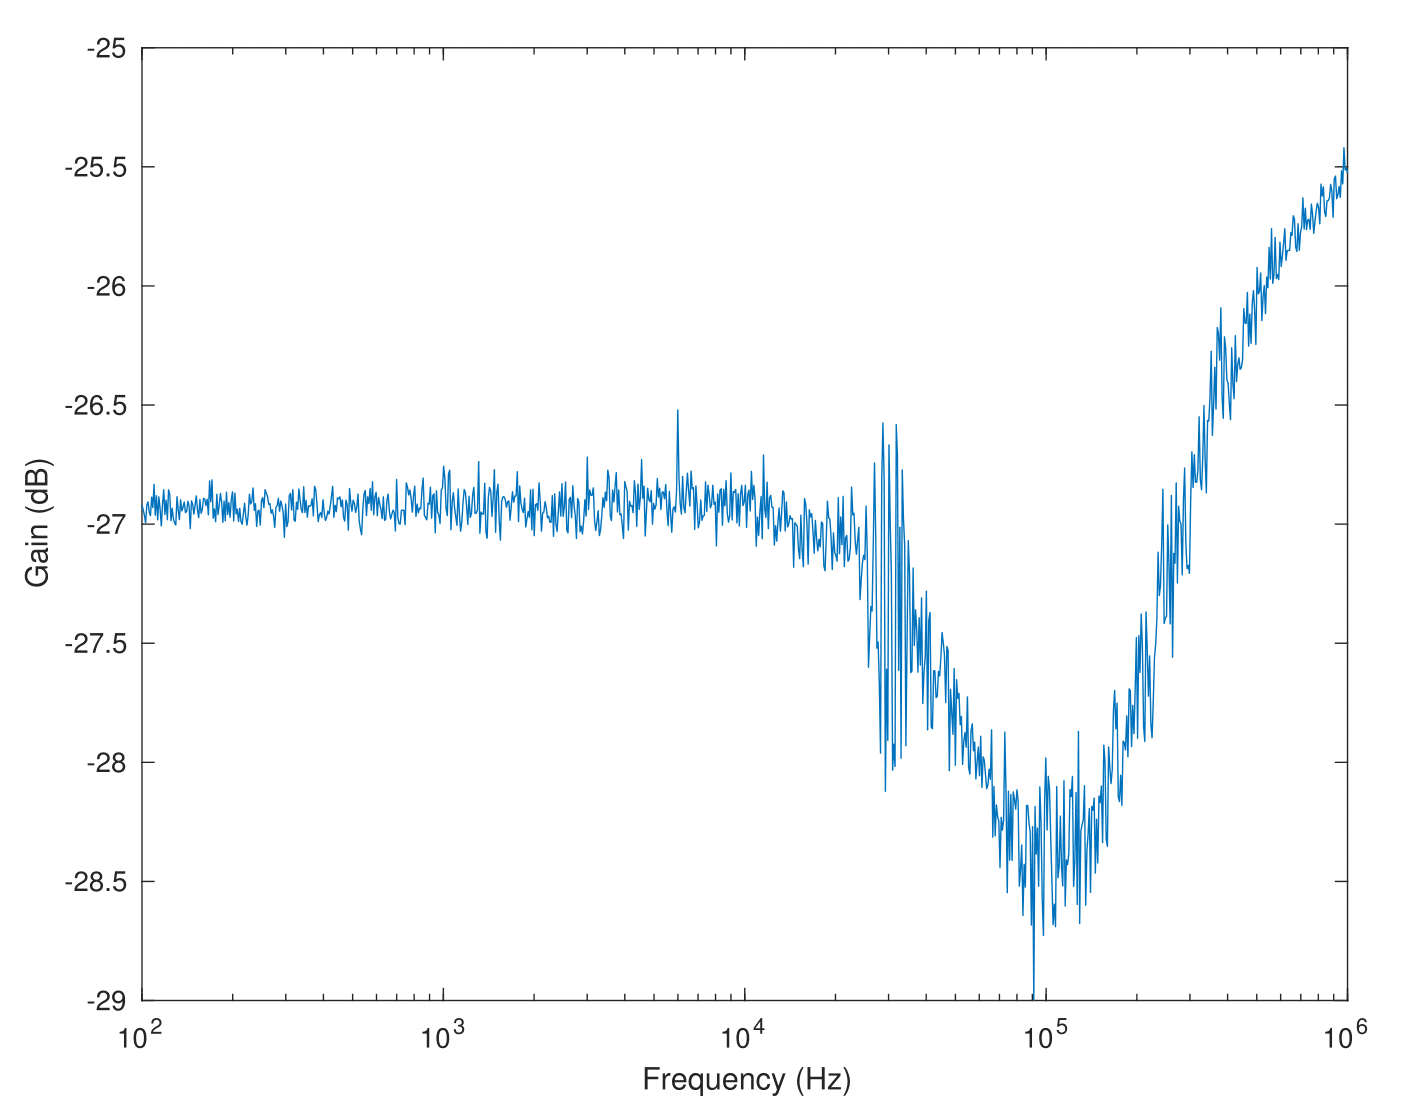
\includegraphics[width=\textwidth]{ExperimentalImplementation/Acm_resist_single_ended_100m_simple.png}
        \caption{Acm, single ended}
        \label{fig:blue_led}
    \end{subfigure}
    \caption{Common mode gain, Acm at 100mV, simple resistive load}
    \label{fig:Acmressimple}
\end{figure} 

The measurement was repeated for 1V as well, which can be seen in Figure \ref{fig:resloadAcm1Vsimple} 

\begin{figure}[H]
    \centering
    \begin{subfigure}[b]{0.45\textwidth}
        \centering
        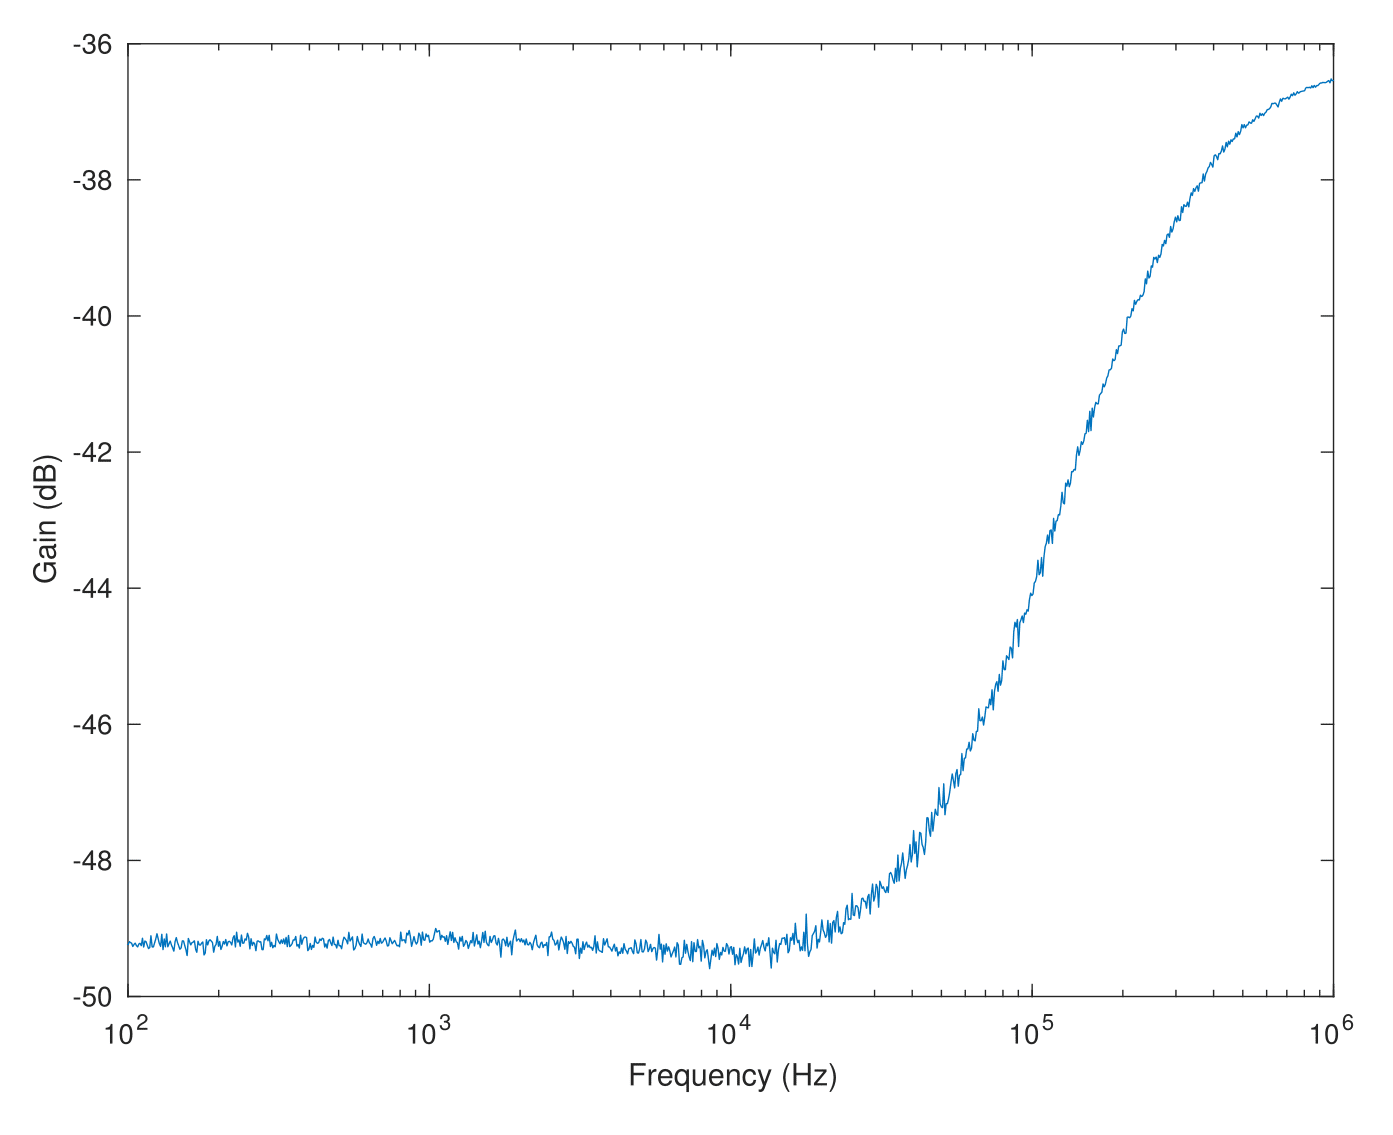
\includegraphics[width=\textwidth]{ExperimentalImplementation/Acm_double_ended_resist_simple_1v.png}
        \caption{Acm, double ended}
        \label{fig:blue_led}
    \end{subfigure}
    \hfill
    \begin{subfigure}[b]{0.45\textwidth}
        \centering
        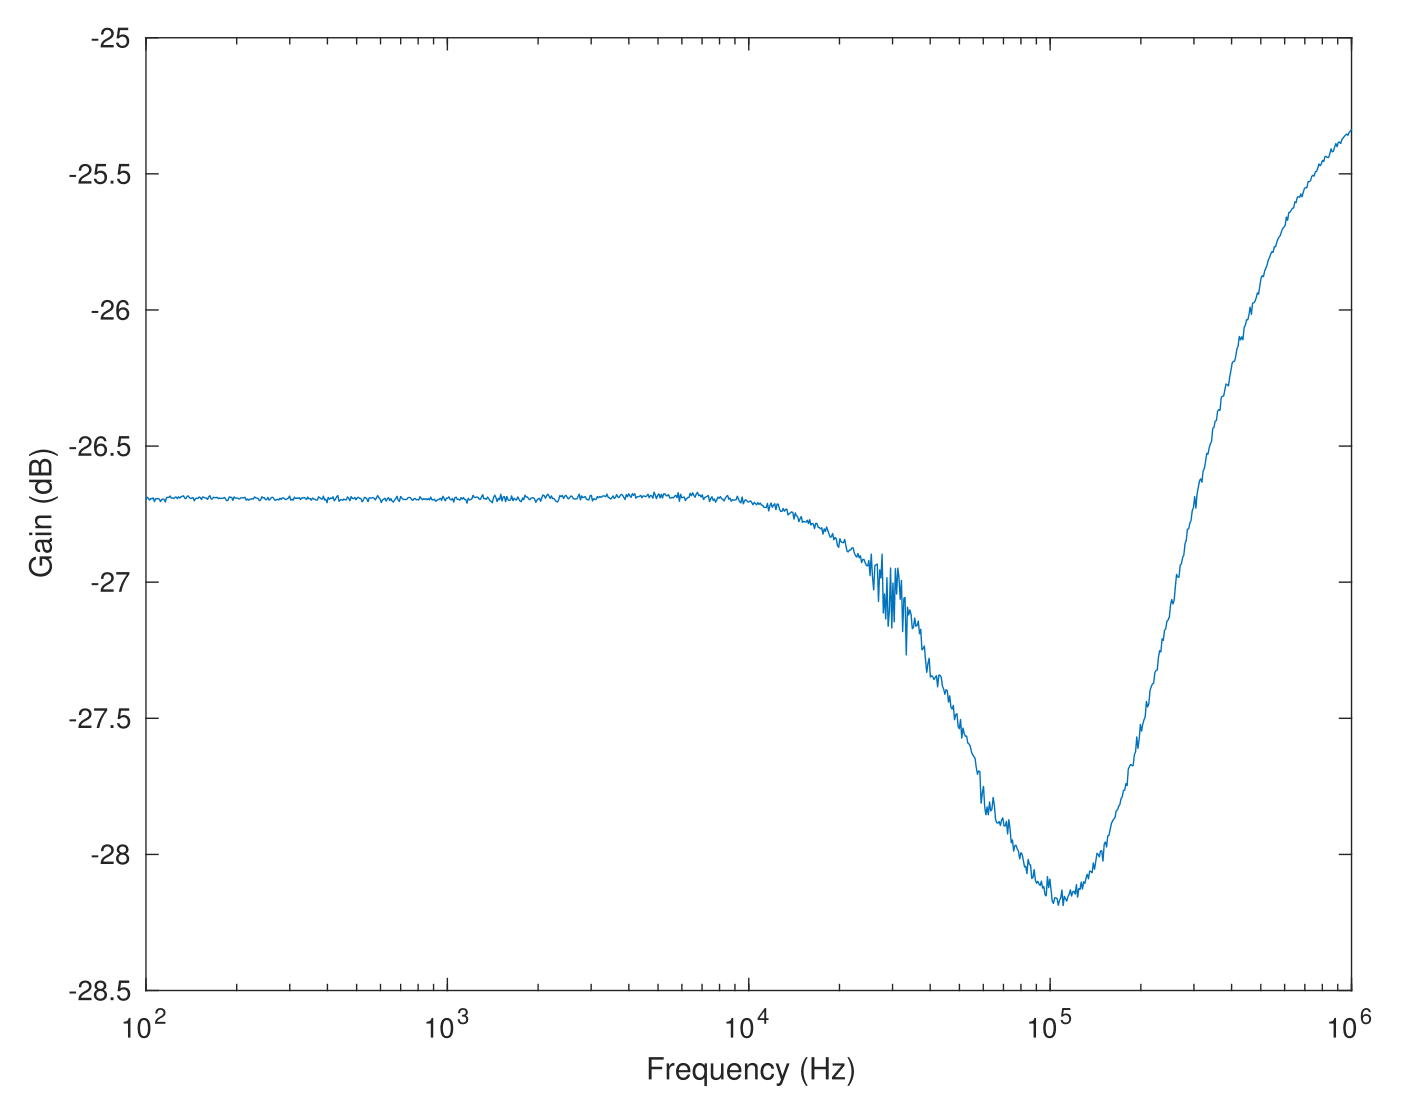
\includegraphics[width=\textwidth]{ExperimentalImplementation/Acm_resist_single_1v_simple.png}
        \caption{Acm, single ended}
        \label{fig:blue_led}
    \end{subfigure}
    \caption{Common mode gain, Acm at 1V, simple resistive load}
    \label{fig:resloadAcm1Vsimple}
\end{figure} 

The 1V clearly had less noise, which is ideal. The trade off, however, is this can saturate the differential gain. From these measurements the CMRR was found and can be seen in Figure \ref{fig:CMRR_simple}.


\begin{figure}[H]
    \centering
    \begin{subfigure}[b]{0.45\textwidth}
        \centering
        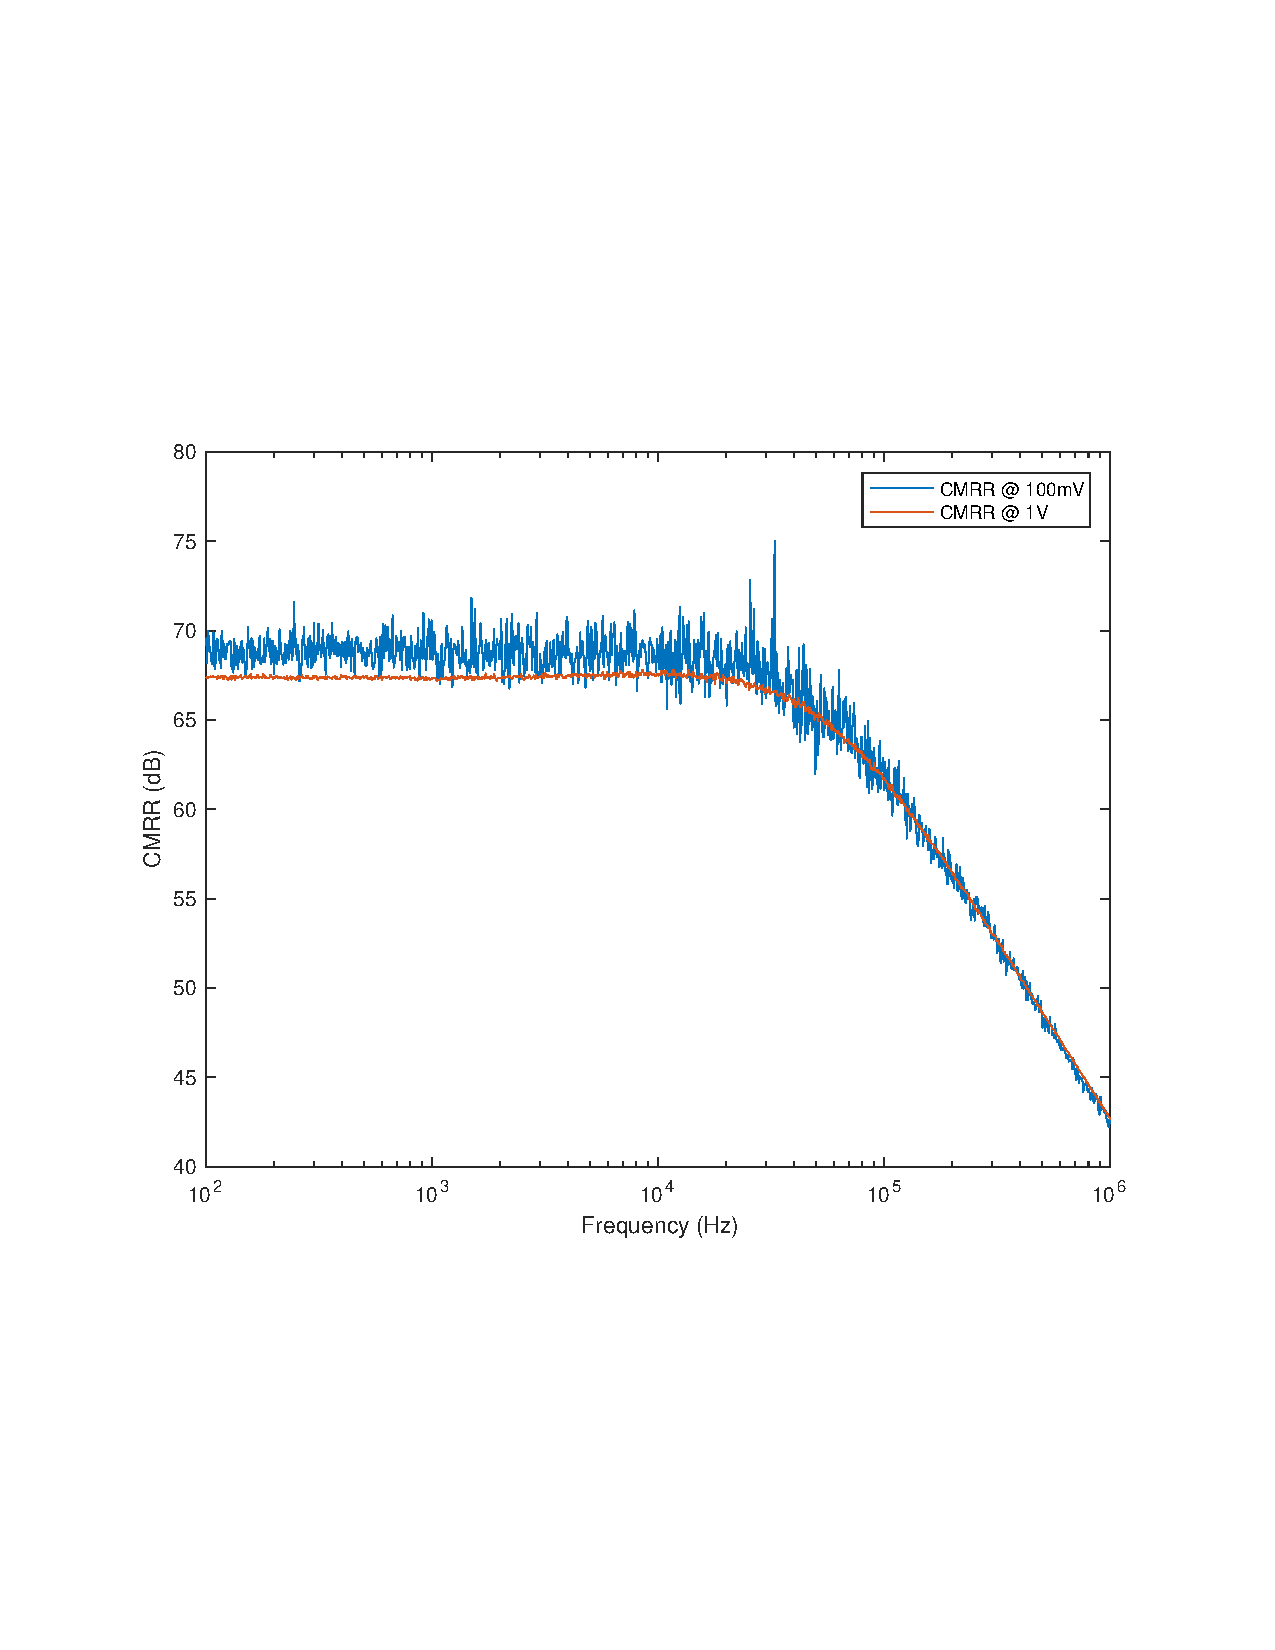
\includegraphics[width=\textwidth]{ExperimentalImplementation/CMRR_resist_simple_double.pdf}
        \caption{CMRR double ended}
        \label{fig:blue_led}
    \end{subfigure}
    \hfill
    \begin{subfigure}[b]{0.45\textwidth}
        \centering
        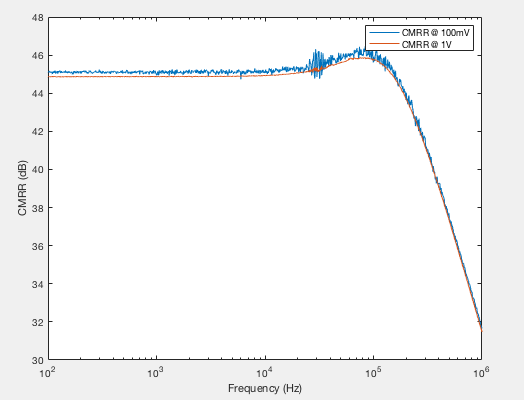
\includegraphics[width=\textwidth]{ExperimentalImplementation/resistive_single_CMRR_simple.png}
        \caption{CMRR single ended}
        \label{fig:blue_led}
    \end{subfigure}
    \caption{Common mode gain, CMRR, simple current resistive load}
    \label{fig:CMRR_simple}
\end{figure} 

As with the cascode, the amplifier performed better with noise rejection at the higher voltage.





%%%%%%%%%ACTIVE LOAD
%%%%%%%%%%
%%%%%%%%%%


\subsection{Active Load Differential Amplifier}
The active load was constructed using PMOS load. The Schematic can be seen in Figure \ref{fig:ActiveLoadExp}. 

\begin{figure}[H]
    \begin{center}
    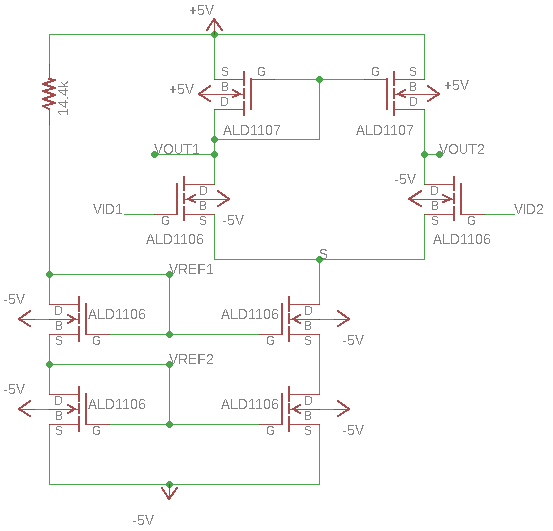
\includegraphics[scale=.85]{ExperimentalImplementation/ActiveLoadedExp.png}
    \caption{Experimental active load differential amplifier}
    \label{fig:ActiveLoadExp}
    \end{center}
\end{figure}

The VTC for the active load can be seen in Figure \ref{fig:activeVTC}.

\begin{figure}[H]
    \begin{center}
    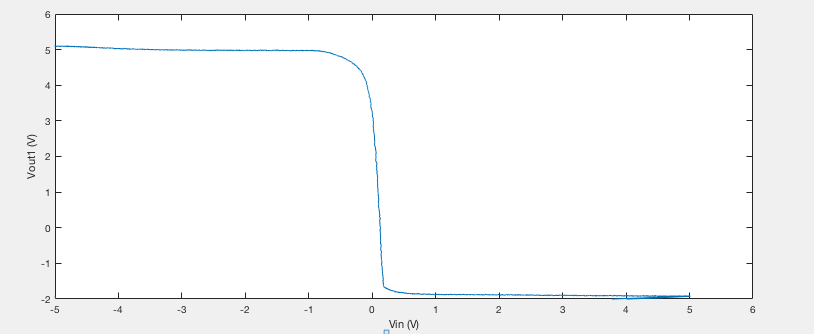
\includegraphics[scale=.45]{ExperimentalImplementation/Active_VTC.png}
    \caption{Experimental VTC of active load}
    \label{fig:activeVTC}
    \end{center}
\end{figure}

The circuit had a much smaller operation range than the resistive load. The differential gain can be seen in Figure \ref{fig:activeAd}.


\begin{figure}[H]
        \center
        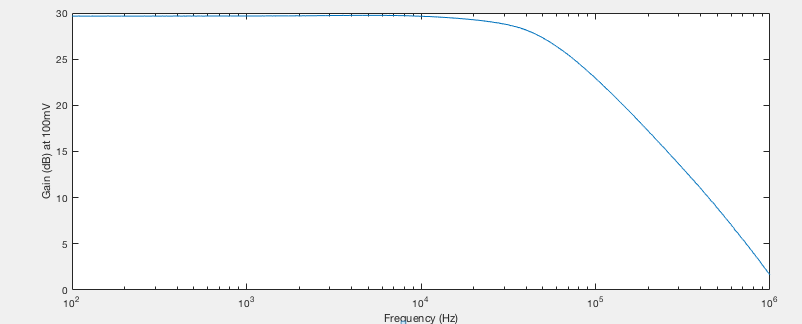
\includegraphics[width=.85\textwidth]{ExperimentalImplementation/Adb_active.png}
        \caption{Ad, double ended}
        \label{fig:activeAd}
 
\end{figure}

The double ended reached higher gain than the single ended. The Acm measured at 100mV  and 1V can be seen in Figure \ref{fig:Acmactive}.



\begin{figure}[H]
    \centering
    \begin{subfigure}[b]{0.45\textwidth}
        \centering
        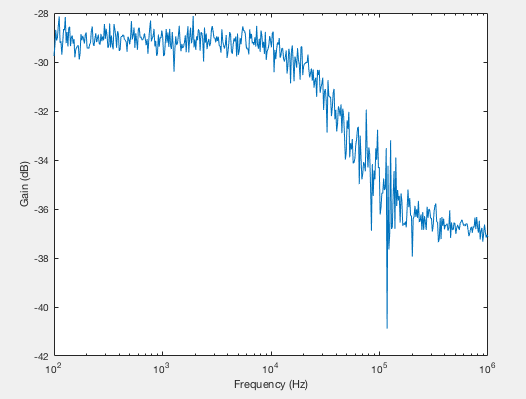
\includegraphics[width=\textwidth]{ExperimentalImplementation/Acm_active_100m.png}
        \caption{Acm, 100mV}
        \label{fig:blue_led}
    \end{subfigure}
    \hfill
    \begin{subfigure}[b]{0.45\textwidth}
        \centering
        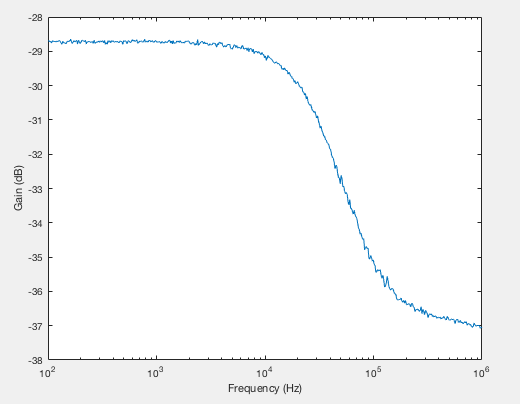
\includegraphics[width=\textwidth]{ExperimentalImplementation/Acm_active_1v.png}
        \caption{Acm, 1V}
        \label{fig:blue_led}
    \end{subfigure}
    \caption{Common mode gain, Acm, active load}
    \label{fig:Acmactive}
\end{figure} 

The commode mode gain was better at the higher voltage. The CMRR can be seen in Figure \ref{fig:CMRRactive}.

\begin{figure}[H]
    \center
    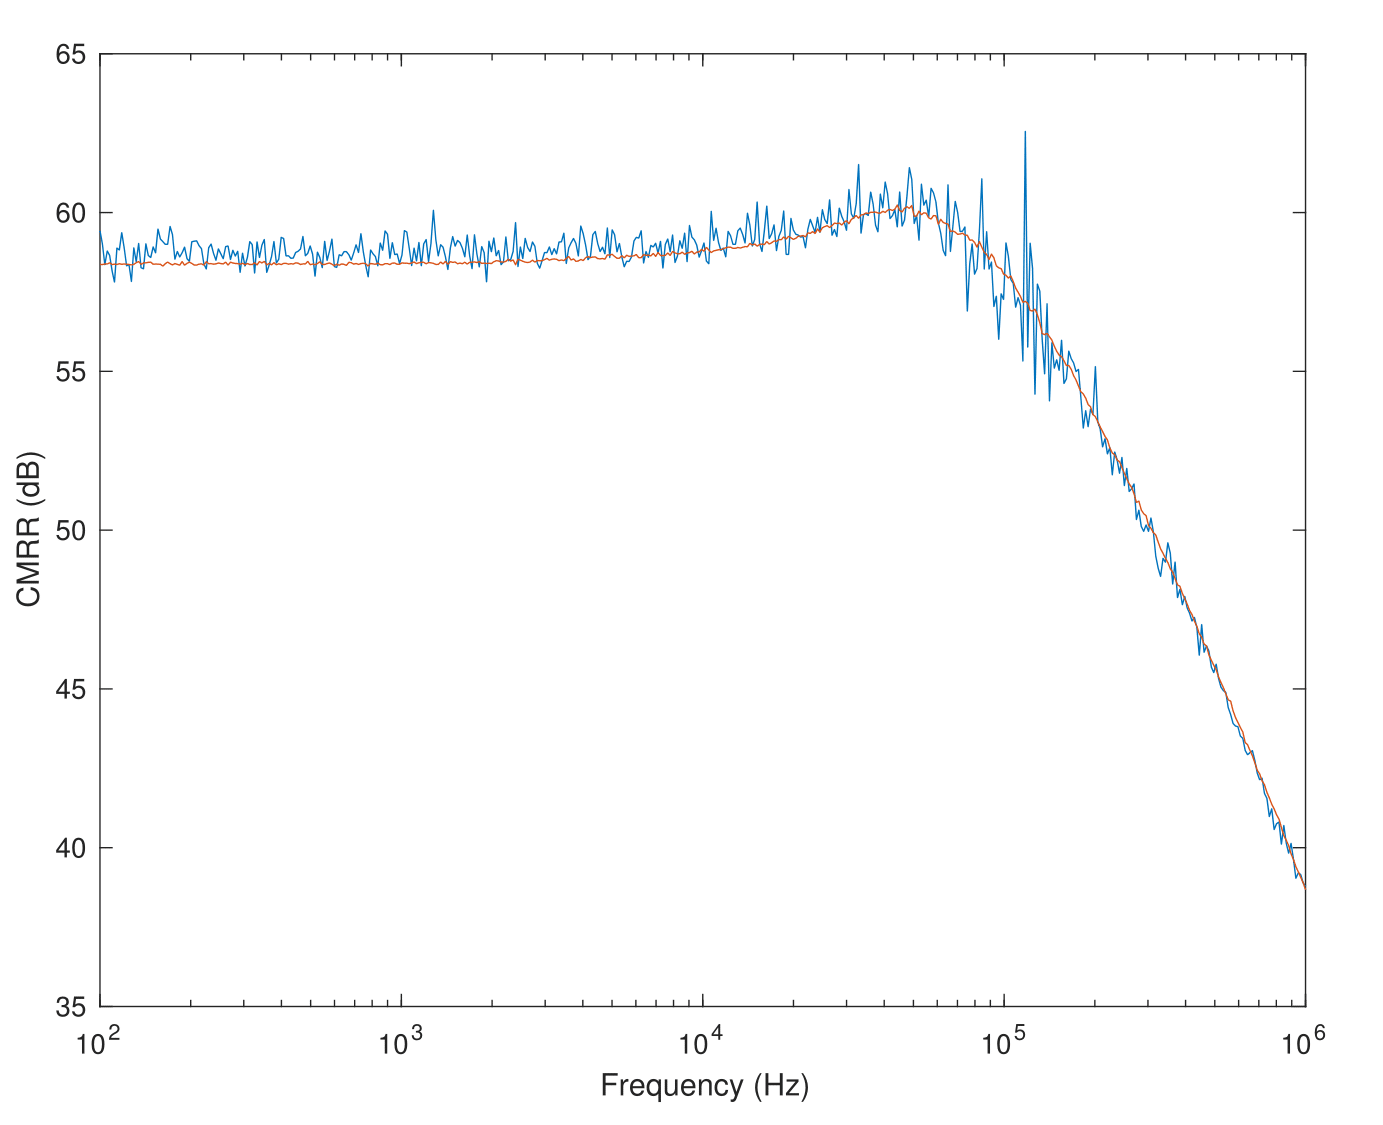
\includegraphics[width=.6\textwidth]{ExperimentalImplementation/Active_CMRR_Both.png}
    \caption{CMRR active load differential amplifier}
    \label{fig:CMRRactive}
\end{figure}

The CMRR was slightly lower than the resistive, but produced a better gain of 30 dB.



\end{document}


